\chapter{Making Sense of Temporal Relationship through User Annotations}
\label{chap:schemaline}

\graphicspath{{Chapter3/figures/}}

\vspace{0.6in}

\begin{figure}[!htb]
	\centering
	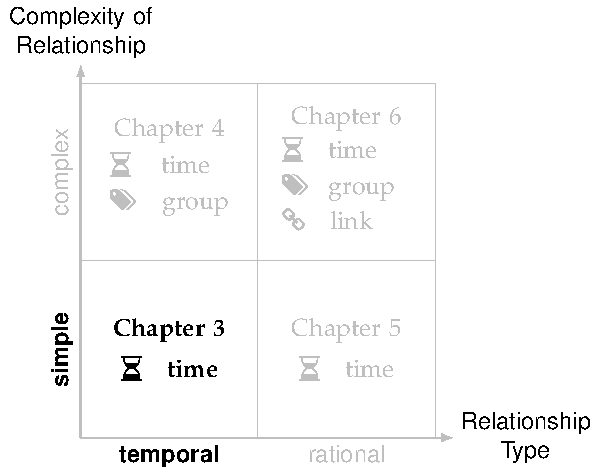
\includegraphics{work-ch3}
\end{figure}

\pagebreak

\blfootnote{Published at the \emph{International Conference on Information Visualization}~\cite{Nguyen2014}.}As the first step toward supporting sensemaking using analytic provenance, this chapter discusses how to explore the \emph{temporal relationship} hidden in the sensemaking process, with a focus on the \emph{intelligence analysis} domain. Intelligence analysts often need to examine thousands of reports to identify potential threats from particular persons or organizations. Visual analytics systems provide automatic analysis techniques to leverage analysts from manual investigation of such high volume of documents. However, the limitation of working memory prevents analysts from holding and managing all discoveries simultaneously. \emph{Annotation} is a technique that can be used to capture high-level thinking and reasoning of analysts throughout their sensemaking processes. Moreover, analysts can organize their annotations to consolidate their thoughts such as in a timeline to represent a story.

\emph{Timeline} is a simple yet powerful technique to visualize time-oriented data, allowing examination of information chronologically and identification of temporal patterns and relationships. However, existing timeline visualization methods are not specifically designed for the dynamic and iterative nature of sensemaking. In this chapter, we introduce a novel timeline visualization -- \emph{SchemaLine} -- to address this issue. SchemaLine allows analysts to construct narratives from their annotations. It produces a compact but aesthetically pleasing layout and provides a set of fluid interactions allowing analysts to perform various sensemaking activities. Our user-centered evaluation shows that the participants found SchemaLine easy to learn and use, and its features effective in supporting the sensemaking activities for which it was designed.

\section{Introduction}
Intelligence analysis is defined as ``the application of individual and collective cognitive methods to weigh data and test hypotheses within a secret socio-cultural context''~\cite{Johnston2005}. To gain a deeper understanding into the sensemaking process in intelligence analysis, Pirolli and Card~\cite{Pirolli2005} conducted a cognitive task analysis with analysts and proposed a process model of sensemaking, which was described earlier in detail in \autoref{sub:lr-sensemaking}. During the sensemaking process, analysts need to read thousands of reports and extract relevant details, organize them in a way that help the analysts to identify patterns and generate hypotheses. This is challenging because of the large number of documents involved and the complex relationship of entities discovered. Visual analytics systems~\cite{Pioch2006,Wright2006,Stasko2007} facilitate intelligence analysis with automated techniques applied to leverage manual investigation of a large document collection. For instance, named-entity recognition techniques~\cite{Nadeau2007} can identify entities (i.e., persons, organizations and locations), and topic modeling techniques~\cite{Blei2003} can extract the main themes discussed. To help analysts manage a large number of discoveries they made during the sensemaking process, the systems allow them to externalize their thoughts through note taking. Analysts are then often supported to freely organized their notes in a way that makes sense to them and facilitates their analyses, such as constructing a timeline of suspicious events.

% Problem of exisiting timelines in sensemaking
\emph{Timeline} is a simple yet powerful technique to visualize time-oriented data~\cite{Tufte1983}, allowing exploration and identification of temporal patterns and relationships in the data. It displays events along the time axis and position them at the time points at which they occur or the time ranges over which they last~\cite{Plaisant1996}. Timelines have been applied extensively in visualizing both raw data and analysis findings for supporting sensemaking. POLESTAR~\cite{Pioch2006} and HARVEST~\cite{Gotz2006} allow analysts to take notes, define new knowledge, and explore them through a timeline visualization. Jigsaw~\cite{Gorg2013} uses timelines to organize extracted named entities, one for each type. Similarly, nSpace2 Sandbox~\cite{SandboxTimeline2012} provides the creation of multiple sub-timelines for visualizing different types of artifacts. However, these timeline visualizations either lack an automatic layout~\cite{Pioch2006} or use an overly-simplistic linear layout~\cite{SandboxTimeline2012}. As a result, the visualization requires significant effort from analysts to manually arrange data elements, making it difficult to detect temporal patterns.

Sensemaking includes dynamic activities centering around the collected data and its explanation~\cite{Klein2003}. Therefore, to support the dynamic nature of sensemaking, timeline visualizations should allow analysts to create and edit temporal structures interactively. Also, the interaction should be intuitive and fluid~\cite{Elmqvist2011} to prevent analysts from extra cognitive effort and distraction. However, existing timeline visualization techniques are mainly designed for presenting a known story rather than revealing and constructing a hidden one interactively.

In this chapter, we introduce a novel timeline visualization -- SchemaLine -- to address the aforementioned issues. More specifically, SchemaLine contributes
\begin{itemize}
	\item A visual design for an interactive timeline that groups annotations into user-determined schemas.
	\item A compact and aesthetically pleasing timeline layout.
	\item A set of fluid interactions with the timeline to support the sensemaking activities described in the Data--Frame model~\cite{Klein2003}.
\end{itemize}
\section{Approach and Requirements}
We began by exploring the literature to get a better understanding of sensemaking in intelligence analysis. As discussed in the Literature Review chapter, \autoref{sub:lr-pcm}, Pirolli and Card describe sensemaking performed by intelligence analysts as a cyclic process including two major loops: the foraging loop and the sensemaking loop. In that model, \emph{schematization} serves as a bridge connecting the two loops and plays an important role in converting raw evidence to rational explanations. Pirolli and Card~\cite{Pirolli2005} suggest that schematization should be supported by a computer-based tool that coordinates events in the dataset to reveal their relationships, and to reduce the effort from analysts in memorizing them. A user study by Kang, Görg and John Stasko~\cite{Kang2011} also shows that timeline is a common choice of participants for organizing related events in an attempt to make sense of them.

% Importance of presenting information in story order
A timeline does not only reveal the temporal relationships of individual findings, but also affects how easily they can be understood. A study by Pennington and Hastie~\cite{Pennington1991} suggests that the presentation order of evidence has a significant impact on making decisions in a court trial. The juror constructs stories based on evidence from witnesses, exhibits and arguments before concluding with the most plausible one. The study shows that participants were most likely (78\%) to convict when the prosecution evidence was presented in story order and the defense evidence was presented in non-story order; whereas, participants were least likely (31\%) to convict when these sets of evidence were presented in the other way round. Therefore, we decided to support \emph{temporal schematization} through interactive visualization.

Based on our understanding about sensemaking in intelligence analysis~\cite{Heuer1999,Pirolli2005}, we set the following requirements for the temporal schematization stage.

\begin{enumerate}
	\item \textbf{Knowledge externalization}. Allow analysts to externalize their thoughts and associate them with relevant raw data.
	\item \textbf{Narrative construction}. Support analysts to create and refine plausible stories from their recorded thoughts.
\end{enumerate}

The first requirement is system dependent and technically straightforward. Note taking or \emph{annotation} is simply implemented in visual analytics systems to allow analysts to record their thoughts. We will discuss it in the context of a specific application system in the evaluation of this chapter (\autoref{sub:sl-evaluation}).

For the second requirement, we propose a system agnostic timeline visualization so that it can be easily integrated into many visual analytic systems. To elaborate on the narrative construction process, we employ various sensemaking activities centering around \emph{data} (annotation/note) and \emph{frame} (schema/story) in the Data--Frame model (\autoref{sub:lr-dfm}). For instance, during sensemaking, an analyst finds some pieces of interesting information. Then, he or she realizes that these pieces mention the same person, thus decides to connect them based on when each event happens in order to reveal the hidden story. Using the terminology of the Data--Frame model, the analyst connects data (the pieces of interesting information) to a frame (the story). To support narrative construction, we decided to enable analysts to perform all sensemaking activities in the Data--Frame model through intuitive interaction with a timeline visualization. 

% Terminology definition
Note that \emph{schema} and \emph{frame} are referred to the same concept: a structure that defines the relationship of data. This chapter focuses on the temporal structure that explains the chronology of events discovered during the sensemaking process. Therefore, a schema or frame can be defined as a chronological sequence of related events. We use \emph{events} instead of general data items or annotations to emphasize on their temporal aspect. To address the second design requirement, we propose the following technical requirements for our timeline visualization.

\begin{enumerate}
	\item \textbf{Event representation}. For each annotation, show its content and its timestamp. This helps remind an analyst what each event is about and when it happens, facilitating the connection of related information.
	\item \textbf{Schema layout}. Easy to follow events within the same schema chronologically. This is essential because an analyst needs to quickly understand and retrieve the schemas he or she created.
	\item \textbf{Data--Frame model}. Enable analysts to perform sensemaking activities described in the Data--Frame model through intuitive interaction.
\end{enumerate}
\section{Visual Design}

\subsection{Event}
An event is represented by a rounded rectangle with a short text inside summarizing its content. The width of an event rectangle is constrained by a threshold and long text is trimmed to fit into its area. The full content of an event will be revealed when it is hovered. Events can be classified into different categories based on certain criteria. For example, a news article may write about \emph{sport}, \emph{fashion} or both. Small colored badges are added to the left of the text of an event to indicate its categories. The colors are chosen from Qualitative Set 1 of  ColorBrewer~\cite{Harrower2003}. Only around 12 colors can be distinguished simultaneously in the human view~\cite{Munzner2014}. Therefore, only the eight most frequently appeared categories are displayed using the selected colormap; whereas, the rest share a different color. \autoref{fig:event} shows an event with three categories.

\begin{figure}[!htb]
\centering
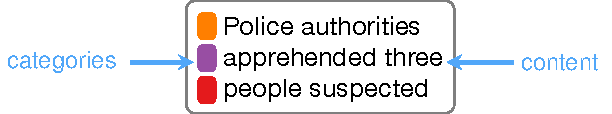
\includegraphics{event}
\caption{Visual representation of event. Text shows the content and colored badges indicate the categories.}
\label{fig:event}
\end{figure}

An event is left-aligned with its temporal value on the time axis. To reduce cluttering, an event is not visually connected to its corresponding point on the axis. Instead, it only appears when the event is hovered. The time axis is shown as a horizontal line at the bottom of all events. It includes two hierarchical temporal scales, changed dynamically according to the range of the visible events. For example, the time axis in \autoref{fig:sl-overview} shows \emph{month} and \emph{day} but they can be switched to \emph{year} and \emph{month} if needed to cover the range of events. This design satisfies the Technical Requirement 1 -- event representation.

\subsection{Schema}
\label{sub:schema}
As discussed in the Literature Review chapter, \autoref{sub:lr-gestalt}, Gestalt principles of grouping are commonly used to show relationships between events, most effectively \emph{connectedness} and \emph{proximity}. Therefore, we also apply these two principles in our design: events belonging to the same schema are located close together, and the background of an entire schema is colored to visually connected all of its events. Spatial grouping needs to be achieved through vertical positioning because the horizontal position of each event is already determined by its temporal information. Locating all events within a schema close together also makes it convenient to follow them chronologically (Technical Requirement 2 -- schema layout).

Munroe's hand-drawn movie narrative charts~\cite{Munroe2009} show the dynamic interactions of characters throughout the movie. Each character is represented as a curved line along a horizontal time axis; and vertical grouping of lines indicates which characters are together at a given interval. Inspired by this technique, we consider a ``schema'' as a ``character line'', connecting all of its events. However, instead of a thin line, we use a thicker path to provide enough space for displaying the content of events and to allow convenient interaction with individual events. For aesthetics, the path is connected rectilinearly, including only horizontal and vertical segments. Also,  all events are constrained by the same height to make the width of the path consistent. \autoref{fig:schema} shows two examples of schema. 

\begin{figure}[!htb]
	\centering
	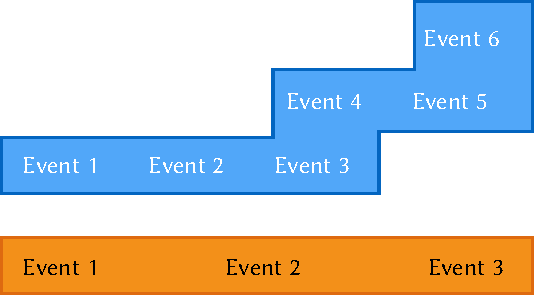
\includegraphics{schema}
	\caption{Visual representation of schema as a colored stripe. Bottom: a simple rectangle connects events that can display in the same row. Top: a rectilinear path connects events that need to locate in different rows.}
	\label{fig:schema}
\end{figure}

Putting it all together, \autoref{fig:sl-overview} shows an example of a complete SchemaLine visualization. The algorithm to produce this is described in \autoref{sec:sl-algorithm}.

\begin{figure}[!htb]
	\centering
	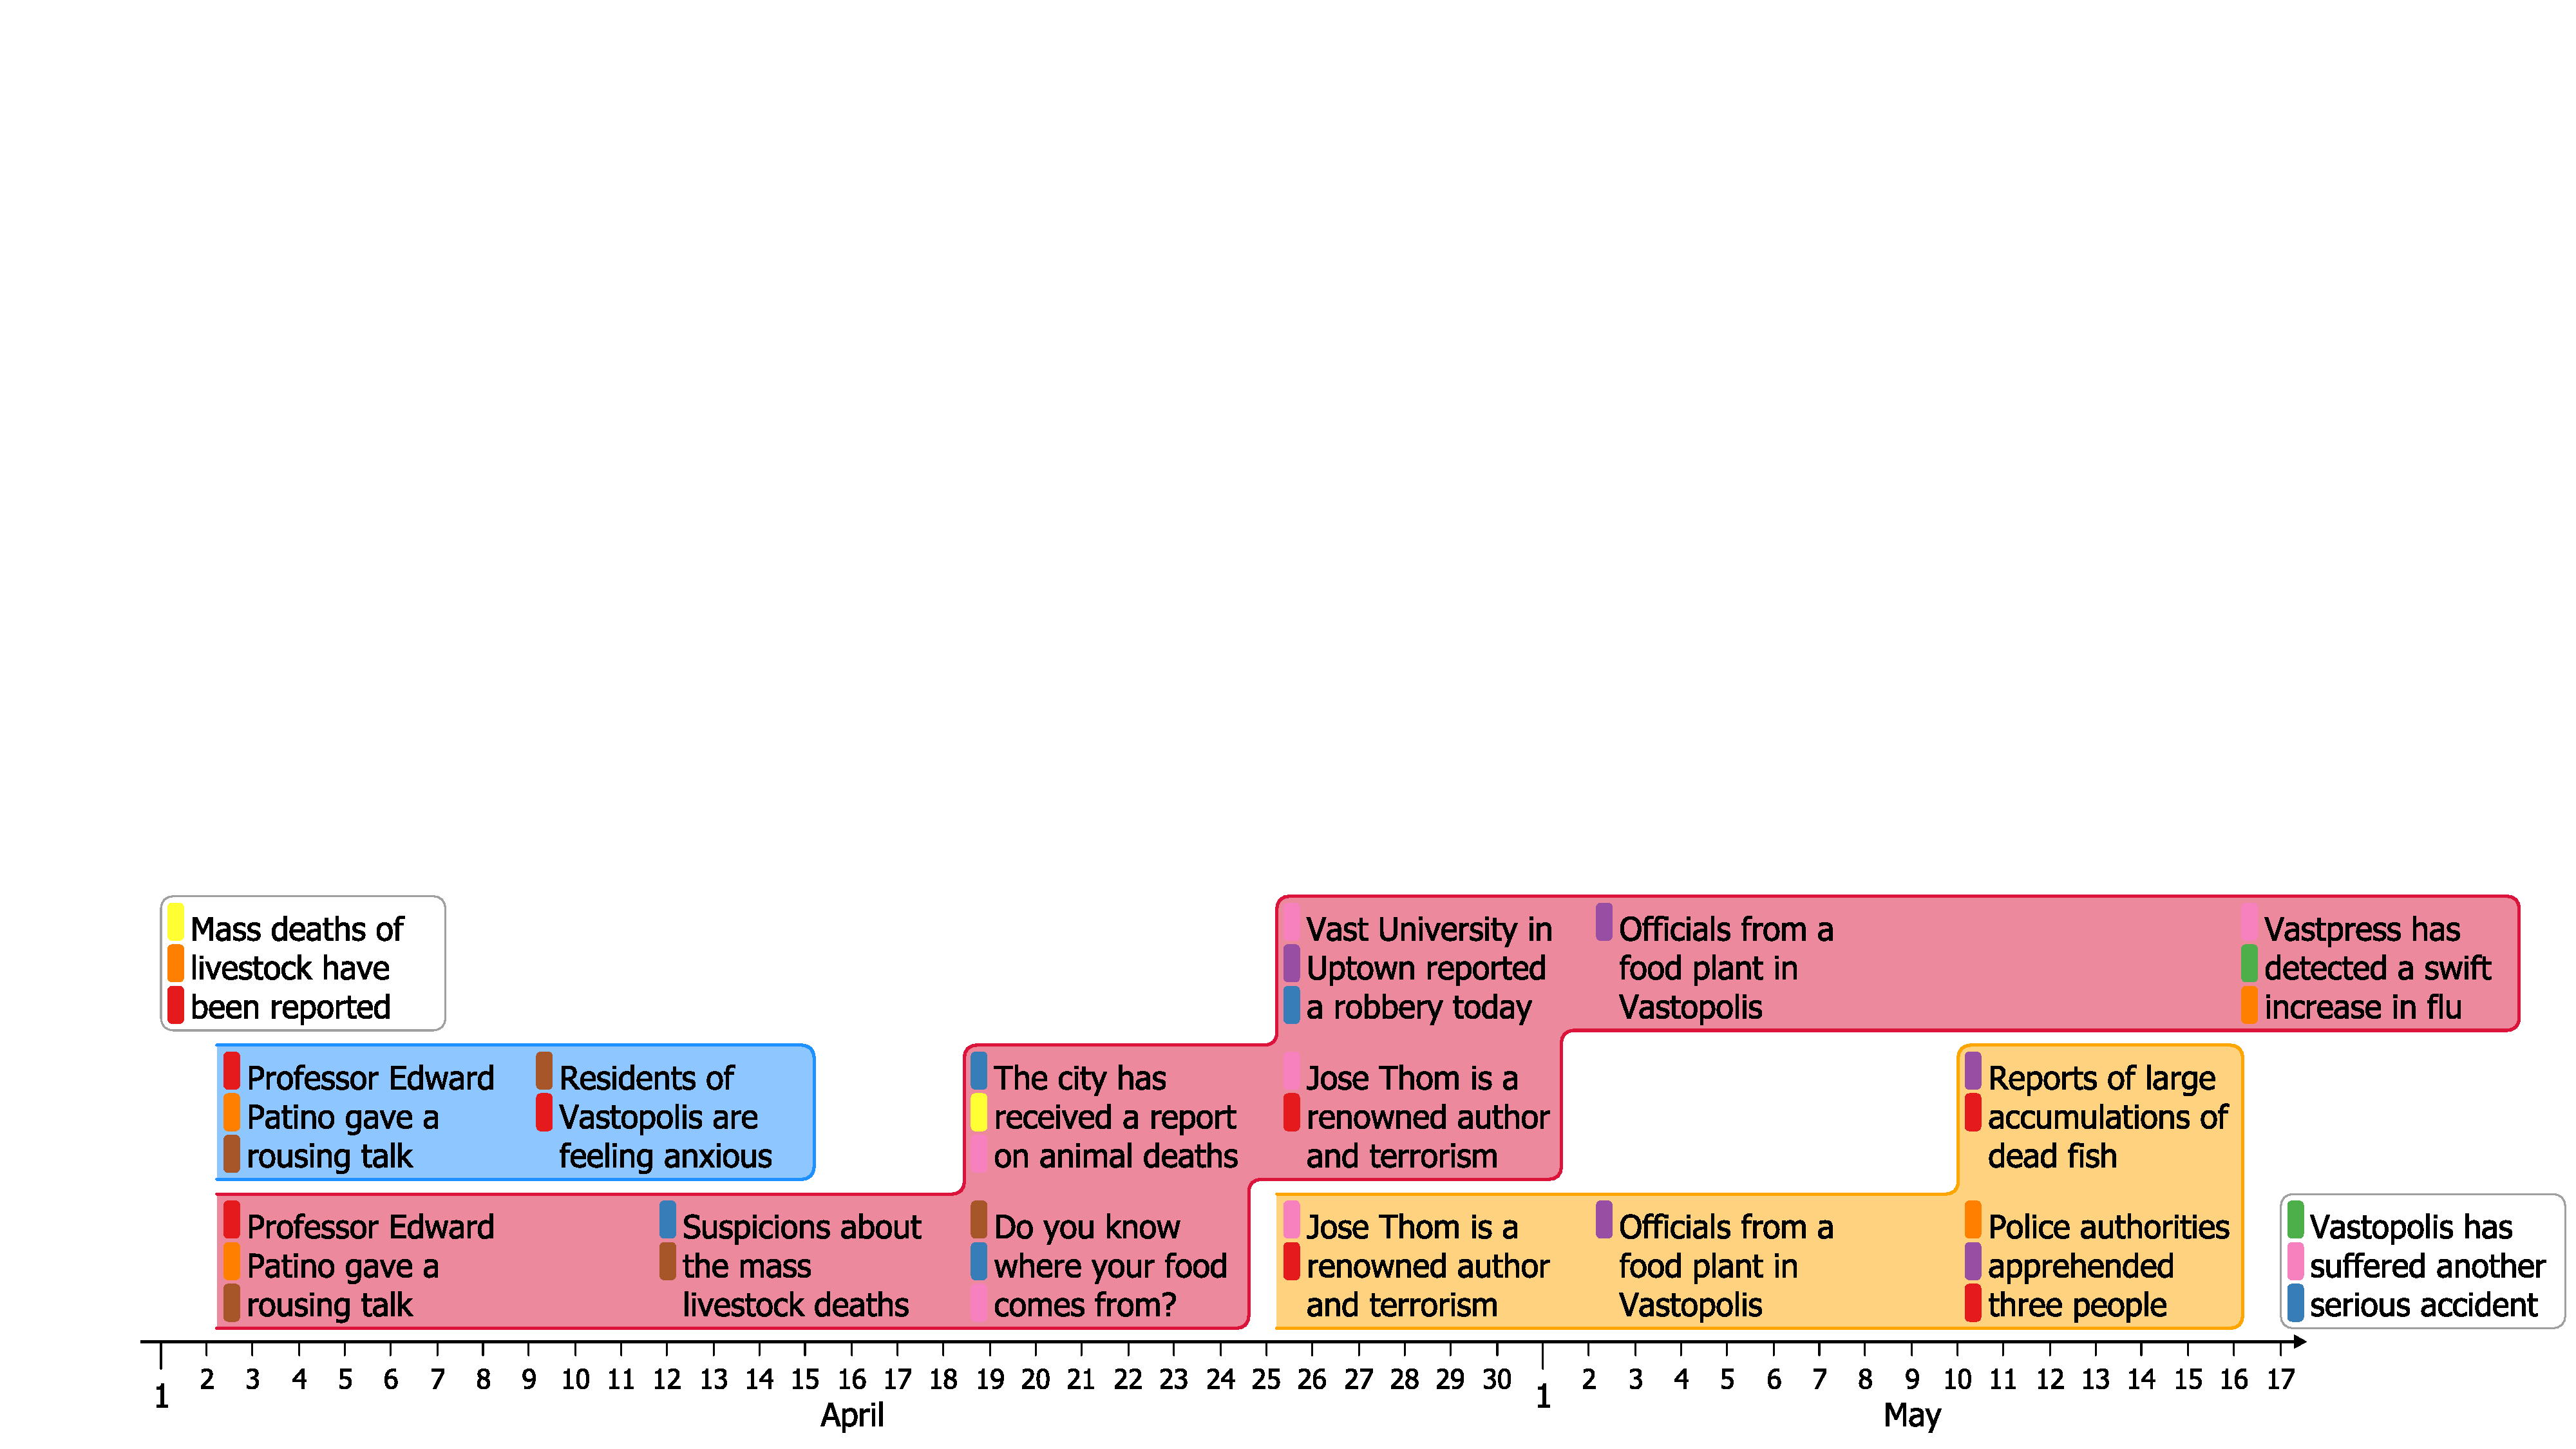
\includegraphics[width=\linewidth]{overview}
	\caption{SchemaLine visualization of annotations. Related ones are connected to form schemas.}
	\label{fig:sl-overview}
\end{figure}

\subsection{Interaction}
To enable analysts to intuitively perform sensemaking activities described in the Data--Frame model (Technical Requirement 3), we follow the design guidelines of fluid interaction proposed by Elmqvist~et~al.~\cite{Elmqvist2011}. More specifically, interactions in SchemaLine 
\begin{itemize}
	\item Produce smooth animated transitions between the state before and the state after an interaction, helping analysts to maintain their mental maps.
	\item Provide immediate visual feedback, enabling analysts to know what is happening and/or what will happen next.
	\item Manipulate directly on the visual representations of events and frames, instead of using extra menus and buttons.
\end{itemize}

During sensemaking, when the analyst recognizes a relationship of events, he or she can group them together and find an account for them (\textbf{connect data and a frame}). This activity is performed by dragging one event and dropping it onto another event, resulting a new frame consisting of these two. While dragging over, a \emph{plus} icon and a rectangle with dashed border surrounding the two events are displayed to indicate that a new frame will be created. 

The analyst can also \textbf{elaborate the frame} by adding more relevant events. This is simply executed by dropping events onto the colored stripe representing the frame. Conversely, to \textbf{preserve the frame}, the analyst can drag its events and drop them onto void space to remove them from the frame. Appropriate informative feedback is displayed in both cases: a \emph{plus} icon for elaboration and a \emph{minus} icon for preservation. \autoref{fig:add-event-frame} shows an example for elaborating the frame.

\begin{figure}[!htb]
	\centering
	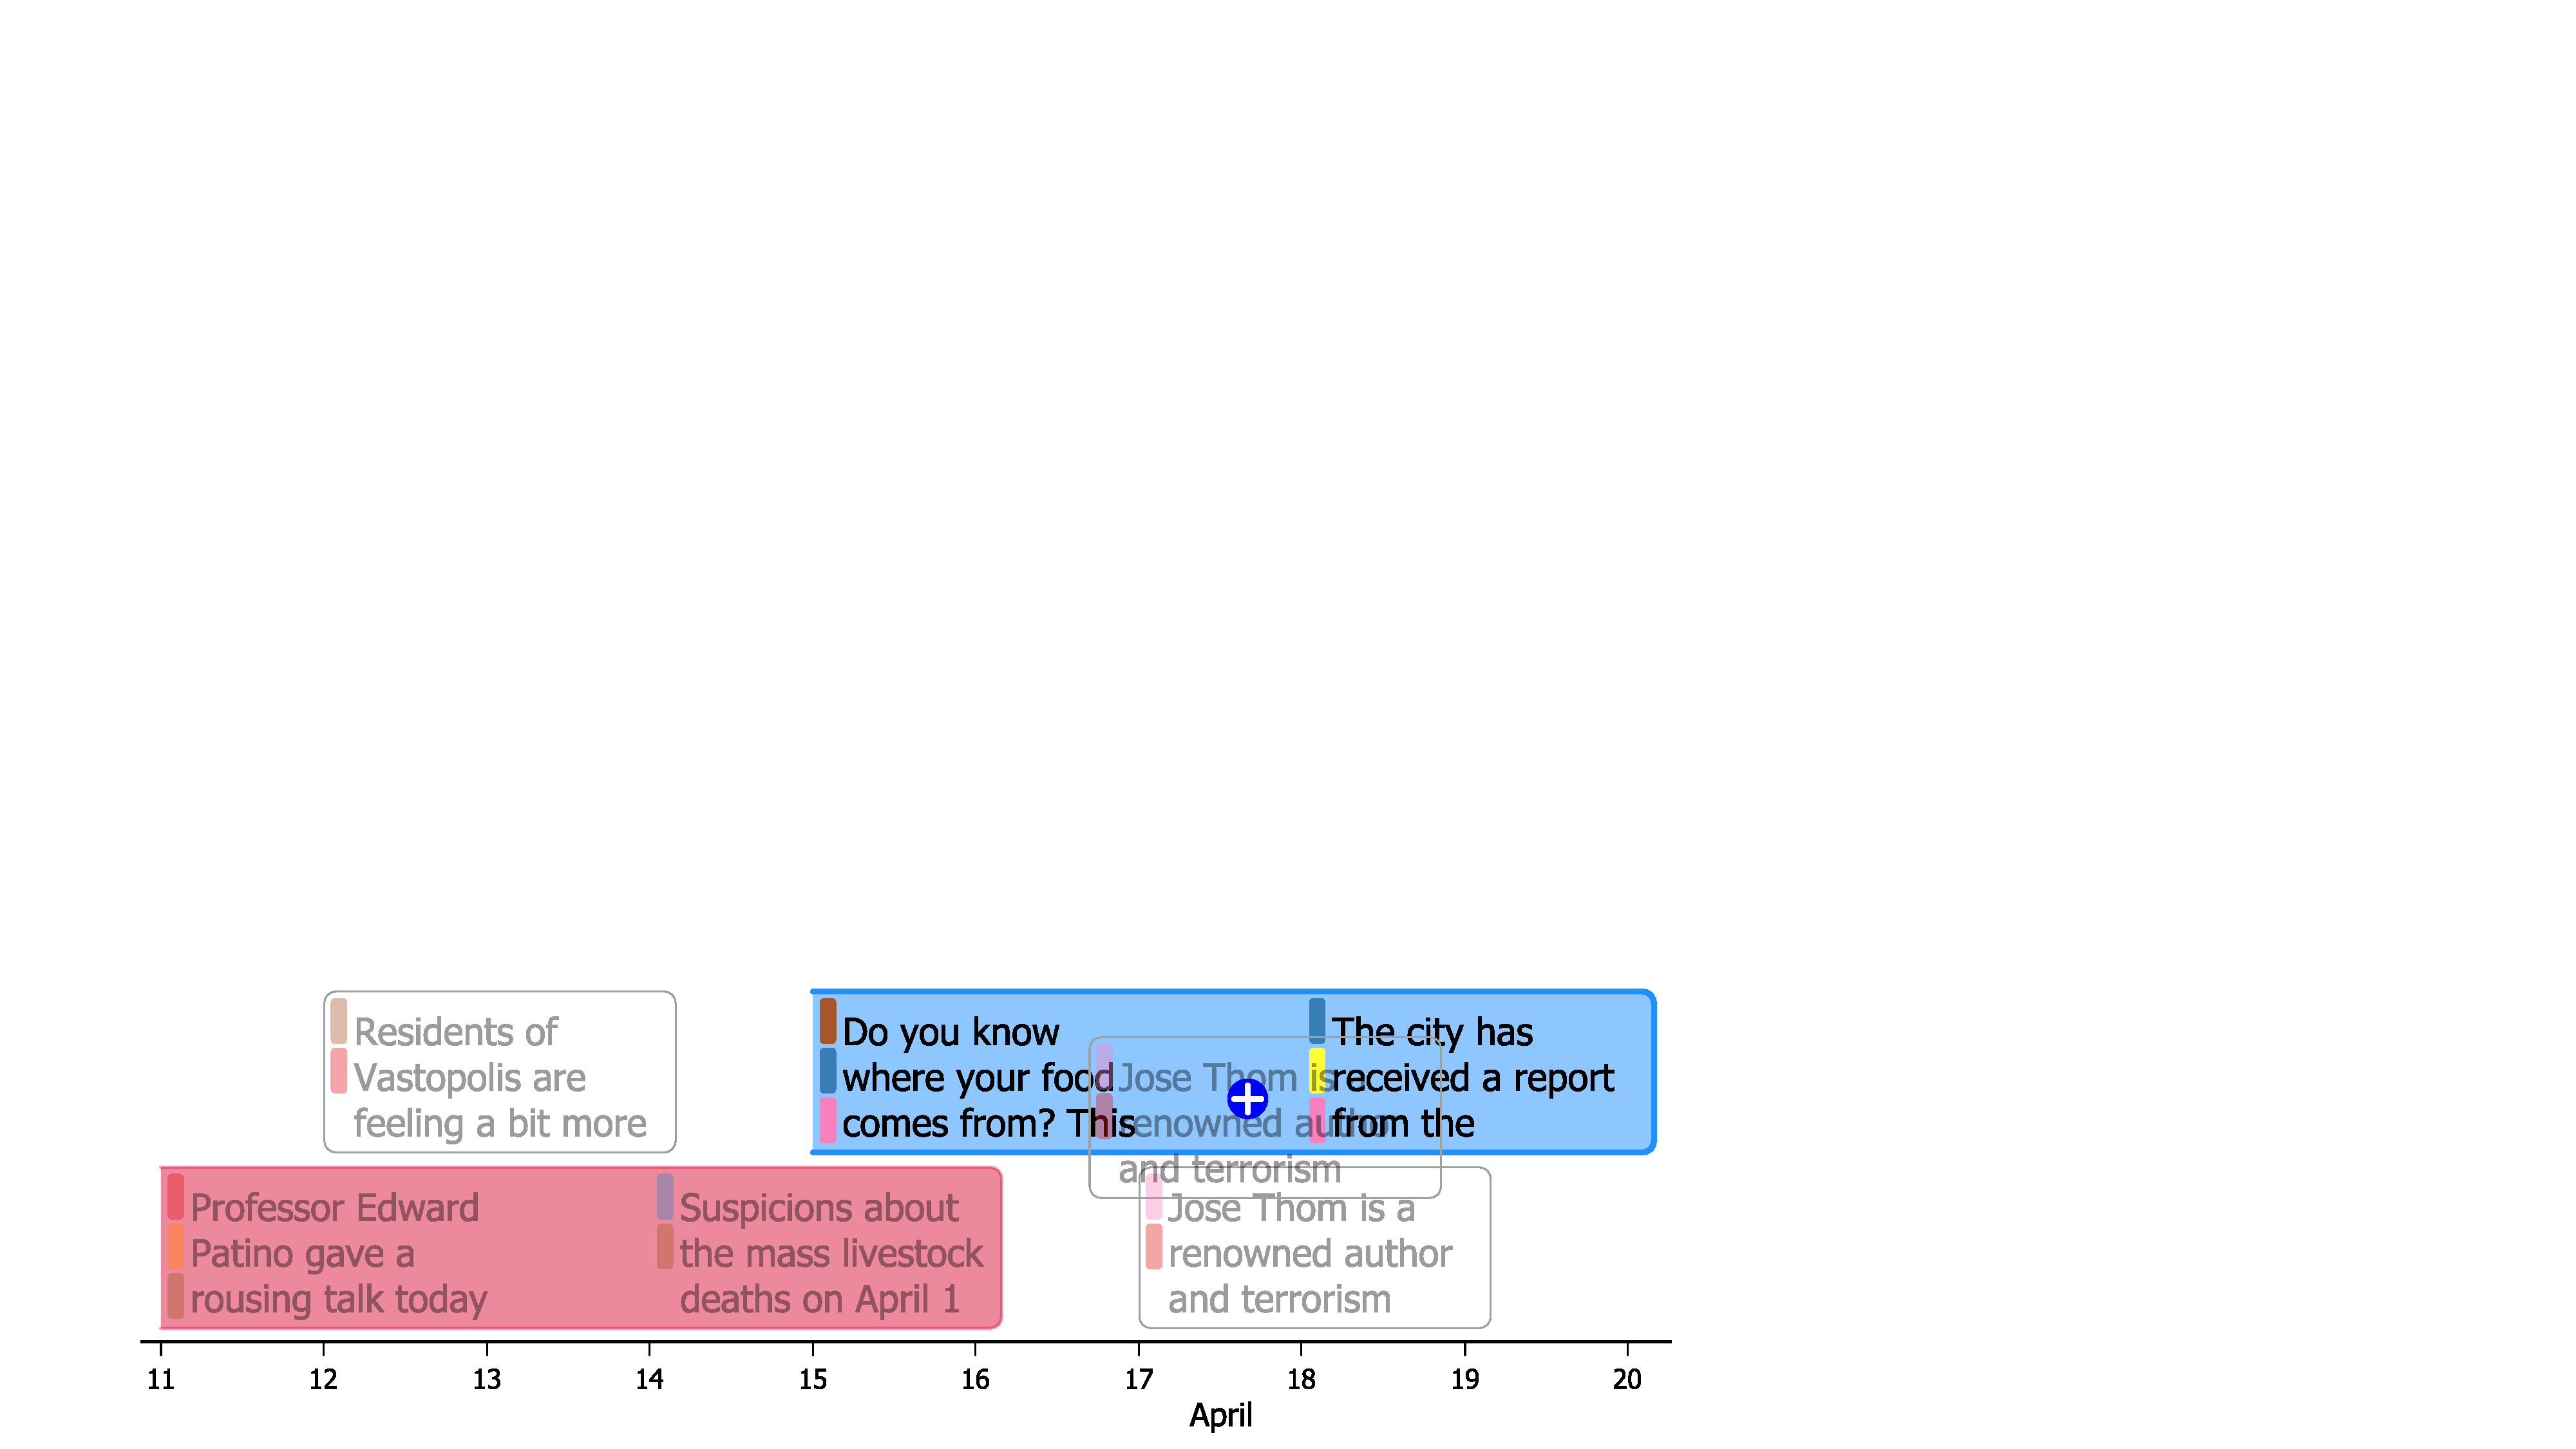
\includegraphics{add-event-frame}
	\caption{Elaborating the frame. Dragging and dropping an event onto the blue stripe to add it to that frame. The plus icon indicates the addition behavior if dropping the event.}
	\label{fig:add-event-frame}
\end{figure}

\textbf{Questioning the frame} occurs when the analyst encounters inconsistencies in data. The temporal distribution of events in the frame may suggest some concerns about the plausibility and completeness of the frame. For example, if a frame about one person contains many events in January and March, but none in February; it may be inferred that some data might be missed. To highlight a suspected event, the analyst can double-click on it with the right mouse button. The text of that event will be rendered in red to indicate that it needs more investigation. 

Depending on experience, the analyst can think of multiple explanations for the same set of data. To support \textbf{comparing multiple frames}, we enable the analyst to duplicate events and construct similar frames. By default, dragging an event from one frame and dropping it onto another frame will move it to the new frame. However, holding the \emph{Control} key while dropping an event will instead copy it to the new frame. Also, when two frames are selected, they will be moved vertically next together to facilitate comparison.

The analyst can remove an event from the timeline by dropping it at the bottom of the time axis. A red \emph{remove} icon is displayed as a visual feedback. While searching for a replacement to account for inconsistent and contrary data (\textbf{reframing}), it could be useful to consider discarded data. To enable that, SchemaLine can redisplay events that were removed earlier with half transparency to distinguish them from existing events.

When the analyst thinks that the existing frame cannot account for its data, he or she may  completely discard it and \textbf{seek a new frame}. The frame can be removed by dropping it onto void space. However, its events still remain in the timeline, enabling the analyst to exploit them. Another interaction could be useful is to combine two sets of events together -- we call it ``merge frames''. This can be performed by dragging one schema and dropping it on top of the other schema.
\section{Layout and Outline}
\label{sec:sl-algorithm}
This section discusses how to produce the SchemaLine visualization such as the one in \autoref{fig:sl-overview}. The layout of schemas is generated before their outlines are computed based on the layout information.

\subsection{SchemaLine Layout}
Based on the technical requirements, the layout should satisfy these conditions: 
\begin{enumerate}
	\item \textbf{Horizontal position}. Along the time axis, events should be located accurately at when they happen, if possible. This is to meet Technical Requirement 1 -- event representation.
	\item \textbf{Relative order}. However, to address scalability, events can be shifted horizontally as long as their relative order is maintained: $x(e_1) < x(e_2)$ if and only if $e_1$ happens before $e_2$, where $x(e)$ is the horizontal position of event $e$.
	\item \textbf{Overlap free}. Events and schemas are not allowed to intersect each other.
\end{enumerate}

To meet these conditions, we design a layout algorithm consisting of the following four steps (\autoref{fig:sl-layout-overview}):
\begin{enumerate} 
	\item Order the schemas vertically based on their number of events.
	\item For each schema, locate its events satisfying the aforementioned requirements.
	\item Compact the schemas following the order computed in the first step.
	\item Locate the remaining events that do not belong to any schemas. 
\end{enumerate}

\begin{figure}[!htb]
\centering
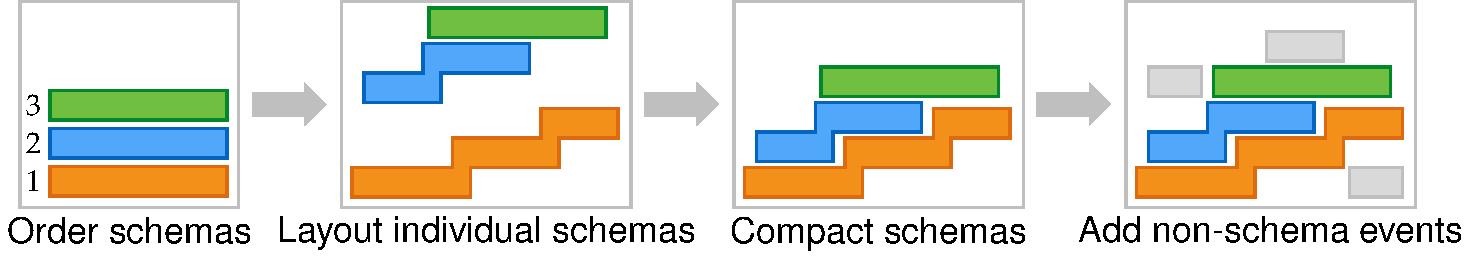
\includegraphics[width=\linewidth]{layout-overview}
\caption[Summary of SchemaLine layout algorithm]{SchemaLine layout algorithm consisting of four steps. First, the vertical order of schemas is computed. Second, the layout of each schema is generated independently. Third, the schemas are compacted based on the computed order. Last, events that do not belong to any schemas are added to the visualization.}
\label{fig:sl-layout-overview}
\end{figure}

\subsubsection{Order Schemas}
As explained in \autoref{sub:schema}, schemas are vertically stacked to apply the \emph{proximity} principle. This step computes the vertical order of all schemas based on their number of events: the schemas with more events are located under the one with less events. This ordering is based on an assumption that larger schemas (in terms of the number of events) are more relevant than smaller ones, thus are located closer to the time axis. If two schemas consist of the same number of events, the one with longer time range is located under.

\subsubsection{Layout Individual Schemas}
\label{sub:layout-schema}
The second step is to produce the layout for each schema. Events that are members of multiple schemas are replicated, allowing the layout of each schema to be generated independently. Events within a schema are sorted chronologically and added to the timeline in that order. Because all events have the same height, only the row level and horizontal position of each event are needed to computed as follows. 

Initially, an event $e_i$ is located on the same row as the previous one $e_{i-1}$ and at the position proportional to its temporal value (Condition 1 -- horizontal position). If these two events are separate, $e_i$ stays at where it is. Otherwise, two cases will be considered. First, if $e_i$ happens at the same time as $e_{i-1}$, it will be located on the upper row and at the same horizontal coordinate as $e_{i-1}$. Second, $e_{i-1}$ is tentatively shifted to the left to make space for $e_i$, as discussed next. If the shift is unsuccessful, $e_i$ will be located in the upper row as in the first case.

\paragraph*{Shifting Events}
To accommodate more events, the accuracy of the horizontal positions of events can be sacrificed. An event can be shifted horizontally to the left to make space for other events. However, an event should not be shifted too far from its accurate position to avoid misinterpretation from analysts. We set that shifting limit to the width of the event so that the event rectangle still covers its time point on the time axis and provides a reasonable indication of its accurate position. 

During shifting, it is essential to make sure that events do not overlap each other (Condition 3 -- overlap free). Considering an event $e_{i-1}$ is shifted to make space for $e_i$, if it overlaps with another event $e_{i-2}$, then $e_{i-2}$ should be shifted as well. Eventually, all events located on the way of the movement should also be shifted. It is also essential to make sure that the relative order between events is still correct after shifting (Condition 2 -- relative order). Otherwise, events with wrong order need to be shifted as well to reestablish the correct order. Note that if two events happen at the same time, they must be located at the same horizontal position. 

\autoref{fig:layout-schema-example} illustrates the layout algorithm for one simple schema.

\begin{figure}[!htb]
	\centering
	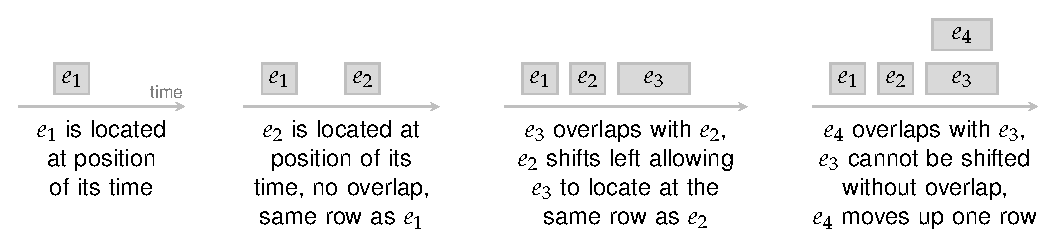
\includegraphics[width=\linewidth]{layout-example}
	\caption[Example of Schema layout algorithm]{Example of Schema layout algorithm. Four events $e_1$, $e_2$, $e_3$ and $e_4$ are added chronologically.}
	\label{fig:layout-schema-example}
\end{figure}

\subsubsection{Compact Schemas}
This third step stacks schemas in the order computed in the first step to produce an overlap-free visualization. However, to make the layout more vertically compact, it is unnecessary to strictly located schemas in that order. Schemas are processed based on the computed order, starting at the bottom row and moving upward. A schema stops when it does not overlap with previously located schemas. In the worst case, it will be located above all other schemas.

\subsubsection{Add Remaining Events}
This last step allocates events that do not belong to any schemas. Events are sorted chronologically and processed in that order. The ideal horizontal coordinate of an event is the position proportional to its temporal value; however, it can also be shifted using the \emph{shifting} method described earlier in \autoref{sub:layout-schema}. An event begins at the bottom row and moves upward until it does not overlap with any other schemas or events after possible shifts. 

\subsection{Schema Outline}
In this section, we describe a process to produce a polygonal outline covering all the event rectangles of a schema. Only horizontal and vertical line segments are used to keep the outline simple yet aesthetic as in \autoref{fig:schema}. The \emph{polygonal path} $P_n$ of a schema that contains $n$ event rectangles $R_1, R_2, ..., R_n$, ordered from left to right, is determined as follows:
\[
P_n=
\begin{cases}
R_1, & n=1 \\
P_{n-1} \oplus R_n, & n > 1
\end{cases},
\]
where $\oplus$ is an operator that appends a rectangle to a polygonal path. As described in the layout of individual schema (Section \ref{sub:layout-schema}), when a new event is added to an existing schema, it has the same row as the previous event (\autoref{fig:outline-right}) or one row higher (\autoref{fig:outline-up}). To produce an aesthetically pleasing path, two other special cases are also considered as described in \autoref{fig:outline-up-one} and \autoref{fig:outline-up-two}. Technically, a path is represented by a list of vertices and is updated when new events are added. \autoref{fig:sl-outline} illustrates how these vertices are updated, added or unchanged for all four those cases.

\begin{figure}[!htb]
	\centering
	
\includegraphics{outline-legend}\bigskip\\
	\subcaptionbox{\label{fig:outline-right}$R_3$ is on the right side of the path.}{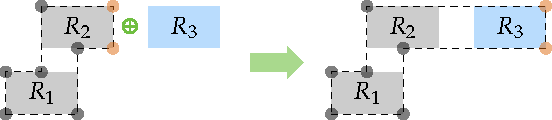
\includegraphics{outline-right}}
	
	\vspace{.5\baselineskip}
	
	\subcaptionbox{\label{fig:outline-up}$R_3$ is on top of the path.}[.43\linewidth]{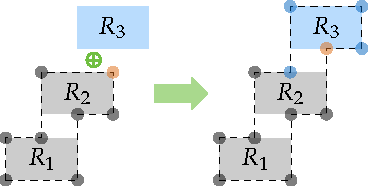
\includegraphics{outline-up}}
	\hfill
	\subcaptionbox{\label{fig:outline-up-one}Left of $R_3$ is a bit greater than left of $R_2$.}[.26\linewidth]{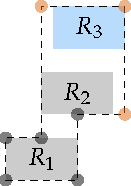
\includegraphics{outline-up-smoothing}}
	\hfill
	\subcaptionbox{\label{fig:outline-up-two}Right of $R_3$ is shorter than right of $R_2$.}[.26\linewidth]{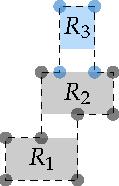
\includegraphics{outline-up-shorter}}
	\caption[Rectangle appended into a polygonal path]{Four cases when a new rectangle \colorbox{f2!40}{$R_3$} is appended \textcolor{ForestGreen}{$\pmb{\oplus}$} to a polygonal path -- representing by a dashed polygon. Vertices of the path are colored coded to describe how they are maintained.}
	\label{fig:sl-outline}
\end{figure}

After producing a rectilinear path, all corner bends are made rounded as in \autoref{fig:sl-overview}. The path is filled with the same stroke color but less transparency to make the border stand out with a darker hue. The beginning of the path does not have the border to indicate the flow of events within the path. 
\section{Evaluation}
\label{sub:sl-evaluation}
SchemaLine was integrated into an existing visual analytics system to evaluate its usefulness in making sense of temporal relationship in intelligence analysis. The integration will be discussed next and followed by a sensemaking case study.

\subsection{Application}
% Overview of INVISQUE
We integrate SchemaLine into INVISQUE~\cite{Wong2011} -- a visual analytics system designed for interactive exploration of text documents. INVISQUE provides full-text search and organizes the search results into a two-dimensional canvas, with each dimension representing a configurable attribute. For example, it may be useful to order academic articles horizontally by publication date and vertically by citation count. Search results are shown as a cluster of \emph{index-cards}, each representing a document with selected information such as publication title, date, keywords and authors. \autoref{fig:invisque} shows a screenshot of INVISQUE.

\begin{figure}[!htb]
	\centering
	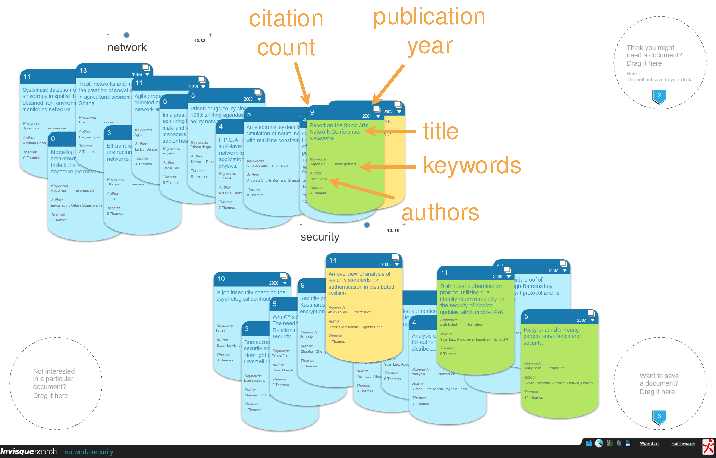
\includegraphics[width=\linewidth]{invisque}
	\caption{INVISQUE interface. It shows two clusters of search results for ``network'' and ``security'' from a publication dataset. Each index-card in a cluster represents an article with meta information displayed on it.}
	\label{fig:invisque}
\end{figure}

% Integration
We add an \emph{annotation} feature to allow analysts to record their thoughts while reading documents. Technically, the association between an annotation and its containing document should be saved for potential provenance retrieval. These annotations are important to analysts, thus are also displayed on the index-cards together with other meta information. The annotations are used  as the input \emph{events} of the SchemaLine visualization. SchemaLine is placed at the bottom of INVISQUE. After the analyst makes a note, or annotation, it is immediately added to SchemaLine as a new event. Double clicking on an event will open the document containing that note as an index-card, enabling the analyst to quickly reexamine the original information source.

% Attribute mapping
The \emph{temporal information} of documents, such as ``publication date'', is initially assigned to that of events, and can be corrected later by analysts. This feature can be useful because the report date is not necessary the same as the date when the event actually occurred. For example, a news article published today can be written about a bomb attack that happened several days ago. The analyst can make the correction by dragging an event with the right mouse button along the time axis and dropping it at the desired date. 

The \emph{label} of an event simply maps to the content of an annotation itself. In INVISQUE, we color code search keywords that contain annotated documents, and use them as \emph{categories} for events. Because a document can be returned from different searches, it can thus contain multiple categories. This mapping provides context for the annotations: what did I search for (the original keyword) and what are other related concepts (other search keywords returning the same document)? This context may help analysts discover interesting patterns through their annotations. \autoref{fig:invisque-schemaline} shows a screenshot of INVISQUE with SchemaLine integrated.

\begin{figure}[!htb]
	\centering
	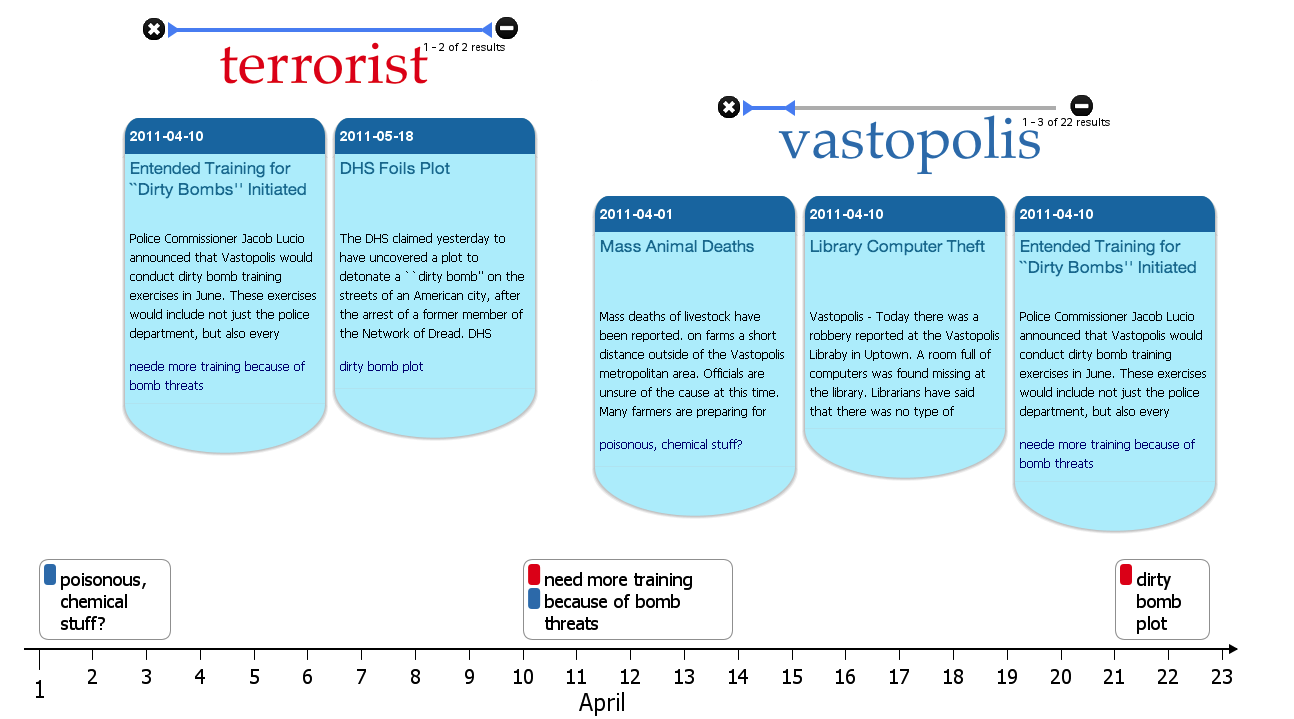
\includegraphics[width=\linewidth]{invisque-schemaline}
	\caption{INVISQUE with SchemaLine at the bottom. The timeline consists of three events, which are notes taken by an analyst. Color coded categories of events indicate keywords that were searched for.}
	\label{fig:invisque-schemaline}
\end{figure}

\subsection{Case Study}

\subsubsection{Design}

\paragraph{Method}
Evaluating the usefulness of SchemaLine in supporting sensemaking can be categorized as \emph{evaluating visual data analysis and reasoning} -- one of the seven scenarios in evaluating information visualization proposed by Lam~et~al.~\cite{Lam2012}. The goal of this evaluation scenario is to explore whether and how a visualization tool supports participants to make sense of the given tasks and generate relevant knowledge. During solving sensemaking tasks, participants may employ various strategies. Their processes and outcomes are also highly context-sensitive, making it difficult to quantify and compare their performance. Therefore, sensemaking evaluations are typically case studies with real-world tasks performed by domain experts. We conducted a case study to explore how SchemaLine supports analysts to solve an intelligence analysis task, focusing on how it enables them to perform sensemaking activities in the Data--Frame model. However, due to a limited access to these resources, we instead use a realistic investigative task with graduate students.

\paragraph{Task}
We used the task from Mini Challenge 3 of the IEEE VAST Challenge 2011~\footnote{\url{http://hcil2.cs.umd.edu/newvarepository/VAST Challenge 2011/challenges/MC3 - Investigation into Terrorist Activity/}}, which requires the participants to identify any imminent threats from the given dataset. We chose this task because it resembles a real intelligence task, demanding analysts to read many documents, extract relevant pieces of evidence and assemble them in order to derive insight and find a reasonable answer to the given question. Also, the solution was provided and well-tested by the community, making it possible to assess participants' performance. The participants were given INVISQUE with SchemaLine integrated to solve the task. 

\paragraph{Dataset}
The original dataset contains more than four thousand news reports, 36 of which are relevant to criminal activities and are manually added by the Challenge committee. Both participants in our pilot test failed to find any imminent threats after one and a half hours. Most of their time was spent on reading long (more than 500 words) but irrelevant documents. The reason could be that INVISQUE does not support text-mining features such as entity extraction, which is crucial in analyzing a large document collection. However, the goal of this evaluation was to assess how SchemaLine can provide additional sensemaking support to INVISQUE rather than assessing INVISQUE itself. Therefore, in the main study, we removed all irrelevant documents that are not part of the ground truth to make the dataset size more manageable. The new dataset only contains the 36 relevant documents, 29 of which are correct answers including five criminal activities: food poisoning (13 documents), hacking (3), dirty bomb (6), arms trafficking (4), and money laundering (3). Other documents are isolated cases, acted as false leads. We expected that participants could complete the task within a reasonable amount of time, without affecting the goal of the study. 

\paragraph{Participants and Procedure}
We were unable to recruit real intelligence analysts for the study. Instead, we recruited three graduate students with different backgrounds:  one in visual analytics (surrogate for visualization expert -- \textbf{P1}), one in law (surrogate for domain expert -- \textbf{P2}), and one in computer network (neutral background -- \textbf{P3}). After being introduced features of INVISQUE and SchemaLine, participants had a chance to practice with a trial sensemaking task for 15 minutes. The main task was followed and lasted for one hour. The participants were asked to report the criminal activities they had discovered with supporting evidence. Semi-structured interviews were followed to gain deeper understanding of the sensemaking processes.

\subsubsection{Results and Discussion}
We first summarize the three sessions and present our collective findings next.

\paragraph{Participant 1}
\textbf{P1} began searching for ``bomb'', examined the search results, and searched for  a refined keyword ``dirty bomb''. He took notes in three documents and then linked these notes together (\emph{connect data and a frame}). He then searched for ``Network of Dread'', which was mentioned in one of documents related to the dirty bomb attack. He took a note in the new returned document and dropped it onto the ``dirty bomb'' schema (\emph{elaborate the frame}). While investigating, he encountered an article about a man carrying a frozen turkey having wires coming out of it, which was suspected as a bomb. At first, he dropped the ``turkey bomb'' note onto the ``dirty bomb'' schema. Then, he wondered whether it was a real bomb. After thinking for a while, he removed it out of the schema (\emph{preserve the frame}). \textbf{P1} found the ``dirty bomb'' attack with 4/6 correct pieces of evidence. \textbf{P1} took many notes in documents related to the ``food poisoning'' case; however, he could not link them together because he said that ``I'm not familiar with bio-attack so I couldn't think of it as a threat''. 

\paragraph{Participant 2}
\textbf{P2} took an overview step before searching. He quickly looked at all 36 document titles to have a glimpse of the dataset as well as to detect potential search keywords. Then he searched for ``animal deaths'', read the results, took notes and grouped them together (\emph{connect data and a frame}). He was satisfied with the evidence he found for that crime and switched to read another interesting article ``Library Computer Left'' he came across. From that, he searched for several related terms such as ``computer'' and ``hackers''. He figured out that a group called ``F-alliance'' stole computers from the library and attempted to hack a bank. He dropped a ``computer stolen'' note on top of a ``bank hacking'' note to form a new explanation for the case (\emph{connect data and a frame}). He found another article related to hacking but he said ``I won't drop it to this group because it's just an announcement from the government about potential threats'' (\emph{preserve the frame}). During further investigation, he created another group of notes related to ``bioterrorism'' and ``Prof. Patino''. Then, when figuring out that the reason of the mass deaths is a spore-forming microbe, which is also mentioned in Prof. Patino's talk, he dropped that new group onto the ``animal deaths'' group to combine all notes together because he thought that they were related (\emph{merge frames}). Observing the order of events in the new group on the timeline, he said ``The equipment of Patino was stolen after the animal deaths report, so they couldn't be used in that case. This is the group of a potential threat in using bioterrorism.'' (\emph{elaborate the frame}). \textbf{P2} found the ``hacking'' case with 2/3 correct pieces of evidence and the ``food poisoning'' case with 9/13 correct pieces of evidence. \autoref{fig:evaluation} shows the computer screen of \textbf{P2} when he reported his findings.

\begin{figure*}[!htb]
	\centering
	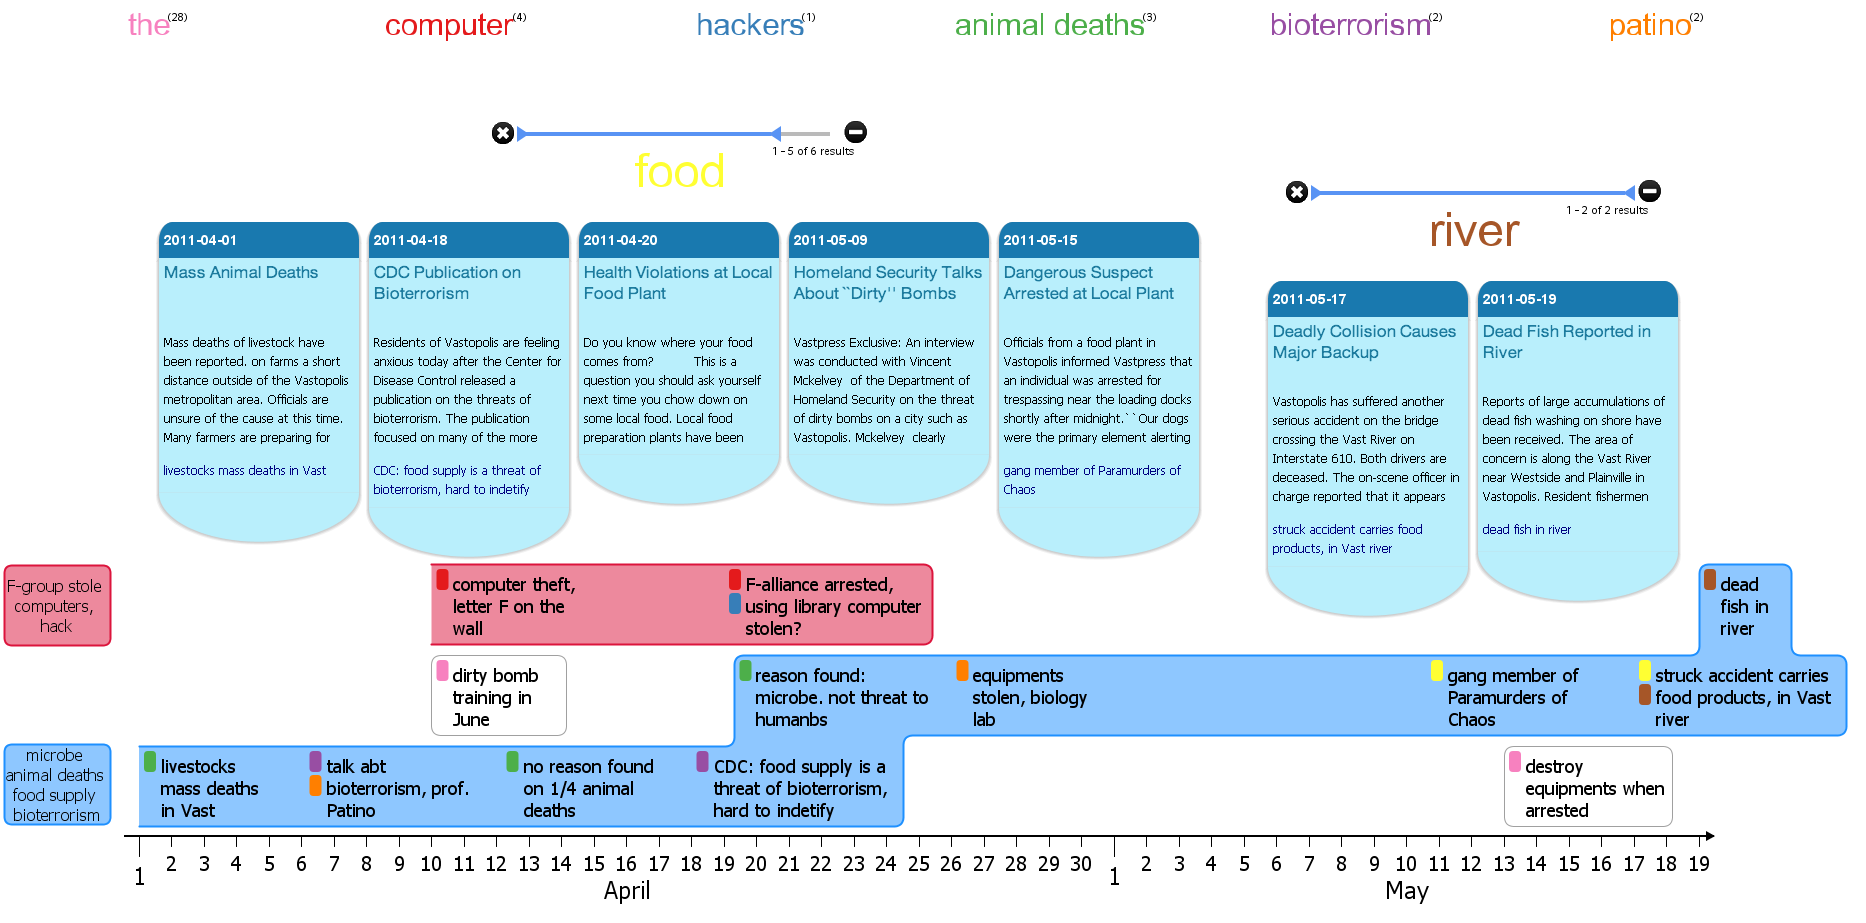
\includegraphics[width=\linewidth]{evaluation}
	\caption{Final screen of participant \textbf{P2}. Top: a trail of his keyword searches, collapsed after being read. Middle: search results in index-card metaphor. Bottom: two schemas containing notes as supporting evidence of criminal activities he found.}
	\label{fig:evaluation}
\end{figure*}

\paragraph{Participant 3}
\textbf{P3} searched for a few keywords related to criminal activities before examining the search results such as ``bomb'', ``terrorism'', ``money'' and ``hack''. He took and group notes about ``money laundering'' together (\emph{connect data and a frame}). Then, he read articles from ``terrorism'' search results. He followed the article content to search for relevant information such as ``Paramurderers of Chaos'' -- a terrorist group. During further investigation, similar to \textbf{P2}, he also combined two groups of notes -- ``Paramurderers of Chaos'' and ``food supply'' -- together when discovering evidence linking the two groups (\emph{merge frames}). When presenting his findings, he shared that SchemaLine prompted him to look for missing information. ``I noticed the gap between these two events [pointing to the timeline]; then I knew I probably missed something there'' (\emph{question the frame}). \textbf{P3} found the ``food poisoning'' case with 6/13 correct pieces of evidence, and a perfect 3/3 pieces of evidence in the ``money laundering'' case. 

\paragraph{Discussion}
% All take notes, build schemas
Three participants applied different sensemaking strategies. \textbf{P1} started with a potential search keyword for criminal activities and kept following the search results. \textbf{P2} initially scanned the titles of all documents to have an overview of the dataset. \textbf{P3} planned ahead what he wanted to search for and sequentially executed it. However, all of them extensively took notes and constructed explanatory frames from them. These frames presented various forms: a concept (bioterrorism), a criminal activity (dirty bomb), a person (Prof. Patino) and a group of people (Paramurderers of Chaos). All participants also employed a variety of sensemaking activities described in the Data--Frame model, supported through fluid interaction in SchemaLine: connect data and a frame, elaborate the frame, question the frame preserve the frame and merge frames.

% temporal sensemaking
All participants appreciated the automatic addition of analyst notes to SchemaLine. \textbf{P1} thought that he would have a problem if the system did not support that: ``I can remember what happened but it was difficult to remember when they happened''. They found that the chronological order of events provides cues to them to construct the story lines. \textbf{P2} shared that he read the news about the robbery at Vastopolis university and the Prof. Patino's talk about bioterrorism. However, he did not have any insight at that time. When looking at his two notes on the timeline, he thought that the extremely expensive equipment in Prof. Patino's lab could be the reason of the robbery. 

% intuitive interface & presentation
All participants commented that the interaction between data and frame was very intuitive. \textbf{P1} said ``I think I don't even need training and still can figure out how it works''. \textbf{P3} appreciated the transition effect when adding or removing notes because ``it helped me to understand what is going on''. All participants were confident while presenting their analyses. \textbf{P3} even opened the original document (double-clicking on the note) several times to highlight the relevant text. He said that the connection between the note and the containing document enabled him to quickly find the information source when needed.
\section{Conclusion and Future Work}
\label{sec:conclusion}

In this paper, we introduced a new timeline visualization, SchemaLine, which is designed to support sensemaking. More specifically, it facilitates the schematization process in the Pirolli-Card model and targets all sensemaking activities in the Data-Frame model. The SchemaLine layout algorithm produces simple, compact, but aesthetically pleasing timeline visualizations. It replaces menu and buttons with fluid user interactions to perform all necessary tasks, and can be integrated within larger visual analytic systems. Our preliminary evaluation suggests that the design of SchemaLine is supportive of sensemaking tasks. It was clearly a helpful aid to users in analysis of the scenario, as evidenced by their usage patterns and feedback. 

As future work, a more formal evaluation would be beneficial -- perhaps even following integration of SchemaLine into a number of different systems, to allow the specific effect to be separated from the rest of the system. In terms of design of the SchemaLine itself, there are a number of improvements that could be added. Shared events between frames could be better visualized (at present, the event is simply duplicated). There are also obvious issues with scalability: while the timeline will scale comparatively well with number of events, it will scale badly with number of frames, since the set of effective qualitative colors is quite small. Other cues such as texture or line style may help with this problem, but to discover this will require further experimentation.